\documentclass[11pt]{article}
\setcounter{tocdepth}{1}

% =====================================
%            пакеты
% =====================================

\usepackage{cmap}
\usepackage[T2A]{fontenc}
\usepackage[utf8]{inputenc}
\usepackage[russian]{babel}
\usepackage{graphicx}
\usepackage{amsthm,amsmath,amssymb}
\usepackage[russian,colorlinks=true,urlcolor=red,linkcolor=blue]{hyperref}
\usepackage{enumerate}
\usepackage{datetime}
% \usepackage{minted}
\usepackage{fancyhdr}
\usepackage{lastpage}
\usepackage{color}
\usepackage{verbatim}
\usepackage{tikz}
\usepackage{epstopdf}
\usepackage{xifthen}
\usepackage{ dsfont }
\usepackage{ wasysym }
\usepackage{ upgreek }
\usepackage{epigraph}
\usepackage{wrapfig}
\usepackage{adjustbox}
\usepackage{float}

\graphicspath{{img/}}
\DeclareGraphicsExtensions{.pdf,.png,.jpg}

\parskip=0em
\parindent=0em

\sloppy
\voffset=-20mm
\textheight=235mm
\hoffset=-25mm
\textwidth=180mm
\headsep=12pt
\footskip=20pt

\pagenumbering{arabic}

\setlength{\parskip}{0.15cm}

\usepackage{indentfirst}

\usepackage{hyperref}
\hypersetup{
	colorlinks,
	citecolor=black,
	filecolor=black,
	linkcolor=blue,
	urlcolor=blue
}

\usepackage{paralist}
\usepackage{cancel}
\usepackage{textcomp}
\usepackage{gensymb}
\usepackage{mdframed}
\usepackage{lastpage}
\usepackage{microtype}
% \usepackage[super]{cite}
\usepackage{fancyhdr}
\usepackage[normalem]{ulem}
\pagestyle{fancy}

\setcounter{page}{1}


\newcommand{\makegood}{
	\ifx\ShortCourseName\undefined
	\gdef\ShortCourseName{\CourseName}
	\fi
	
	% \newcommand\CustomTitle{...} до \makegood для того, чтобы
	% переопределить содержимое титульной страницы до содержания.
	\ifx\CustomTitle\undefined
	\title{\CourseName}
	\maketitle
	\else
	\pagestyle{empty}
	\CustomTitle
	\fi
	
	\tableofcontents
	\pagebreak
	\pagestyle{fancy}
	\pagenumbering{arabic}
	\setcounter{page}{1}
	
	\ifdefined\ENABLEDMATH
	\renewcommand\proofname{\em \bf{Доказательство}}
	\else
	\fi
}

\newcommand{\Section}[2]{
	\newpage % new page
	\stepcounter{section}
	\bigskip
	\phantomsection
	\addcontentsline{toc}{section}{\arabic{section}. #1}
	\begin{center}
		{\LARGE \bf \arabic{section}. #1}\\
		\vspace{0.3em}
		{\Large #2}
	\end{center}
	%\bigskip
	\gdef\SectionName{#1}
	% \gdef\AuthorName{#2}
	% \gdef\DateName{#2}
	
	\lhead{\ShortCourseName}
	\chead{}
	\rhead{\SectionName}
	
	\renewcommand{\headrulewidth}{0.15 mm}
	
	% \ifx\LaconicFooter\undefined
	
	%\rfoot{
	%	%    \topskip0pt\vspace*{\fill}
	%	Автор: \AuthorName
	%	%    \vspace*{\fill}
	%}
	%\renewcommand{\footrulewidth}{0.15 mm}
	% \fi
}

% =====================================
%            математика
% =====================================

\makeatletter
\newenvironment{proof1}[1][\proofname]{\par
  \vspace{-\topsep}% remove the space after the theorem
  \pushQED{\qed}%
  \normalfont
  \topsep0pt \partopsep0pt % no space before
  \trivlist
  \item[\hskip\labelsep
        \itshape
    #1\@addpunct{.}]\ignorespaces
}{%
  \popQED\endtrivlist\@endpefalse
  \addvspace{6pt plus 6pt} % some space after
}
\makeatother

\makeatletter
\newenvironment{solution}[1][Решение]{\par
  \vspace{-\topsep}% remove the space after the theorem
  \pushQED{\qed}%
  \normalfont
  \topsep0pt \partopsep0pt % no space before
  \trivlist
  \item[\hskip\labelsep
        \itshape
    #1\@addpunct{.}]\ignorespaces
}{%
  \popQED\endtrivlist\@endpefalse
  \addvspace{6pt plus 6pt} % some space after
}
\makeatother

\def\eps{\varepsilon}         %
\def\SO{\Rightarrow}          % =>
\def\EQ{\Leftrightarrow}      % <=>
\def\t{\texttt}               % mono font
\def\s{\textsc}               % small capitals (for problem names)
\def\c#1{{\rm\sc{#1}}}        % font for classes \t{NP}, SAT, etc
\def\O{\mathcal{O}}           %
\def\NO{\t{\#}}               % #
\def\edge{\leftrightarrow}    % <->
\def\xto{\xrightarrow}        % ->
\renewcommand{\le}{\leqslant} % <=, beauty
\renewcommand{\ge}{\geqslant} % >=, beauty
\def\xor{\text{ {\raisebox{-2pt}{\ensuremath{\Hat{}}}} }}
\newcommand{\q}[1]{\langle #1 \rangle}               % <x>
\newcommand{\cool}[1]{\mathcal{#1}}

\def\TODO{{\color{red}{\bf TODO}}}

% Должна использоваться вне \document.
\newcommand{\enablemath}{
	\usepackage{amsmath,amsthm,amssymb,mathtext}
	\usepackage{thmtools}
	\usepackage{tikz}
	\usepackage{nameref,hyperref,cleveref}
	
	\ifx\ThmSpacing\undefined
	\def\ThmSpacing{9pt}
	\fi
	
	\ifx\ThmNamespace\undefined
	\def\ThmNamespace{section}
	\fi
	
	\declaretheoremstyle[
	spaceabove=\ThmSpacing, spacebelow=\ThmSpacing,
	% postheadhook = {\hspace{0mm}\newline},
	headfont=\slshape\bfseries,
	bodyfont=\normalfont,
	postheadspace=0.5em,
	]{thmstyle_def}
	
	\declaretheoremstyle[
	spaceabove=\ThmSpacing, spacebelow=\ThmSpacing,
	postheadspace=0.5em,
	]{thmstyle_thm}
	
	\declaretheoremstyle[
	spaceabove=\ThmSpacing, spacebelow=\ThmSpacing,
	headfont=\itshape\bfseries,
	notefont=\itshape\bfseries, notebraces={}{},
	bodyfont=\normalfont,
	postheadspace=0.5em,
	]{thmstyle_cons}
	
	\declaretheoremstyle[
	spaceabove=\ThmSpacing, spacebelow=\ThmSpacing,
	headfont=\bfseries,
	notefont=\bfseries, notebraces={}{},
	bodyfont=\normalfont,
	postheadspace=0.5em,
	]{thmstyle_examp}  
	
	\declaretheoremstyle[
	spaceabove=\ThmSpacing, spacebelow=\ThmSpacing,
	headfont=\ttfamily\itshape,
	notefont=\ttfamily\itshape, notebraces={}{},
	bodyfont=\normalfont,
	postheadspace=0.5em,
	]{thmstyle_remark}
	
	\declaretheorem[numbered=no, name=Теорема, style=thmstyle_thm]{theorem}
	\declaretheorem[numbered=no, name=Сведение, style=thmstyle_thm]{reduction}
	\declaretheorem[numbered=no, name=Определение, style=thmstyle_def]{definition}
	\declaretheorem[numbered=no, name=Задача, style=thmstyle_def]{problem}
	\declaretheorem[numbered=no, name=Гипотеза, style=thmstyle_def]{hypothesis}
	\declaretheorem[numbered=yes, name=Утверждение, style=thmstyle_thm]{statement}
	\declaretheorem[numbered=no, name=Факт, style=thmstyle_thm]{fact}
	\declaretheorem[numbered=no, name=Замечание, style=thmstyle_remark]{remark}
	\declaretheorem[numbered=no, name=Лемма, style=thmstyle_thm]{lemma}
	\declaretheorem[numbered=no, name=Следствие, style=thmstyle_cons]{corollary}
	\declaretheorem[numbered=no, name=Пример, style=thmstyle_examp]{example}
	\declaretheorem[numbered=no, name=Примеры, style=thmstyle_examp]{examples}
	\declaretheorem[numbered=no, name=Свойства, style=thmstyle_cons]{properties}
	\declaretheorem[numbered=no, name=Свойство, style=thmstyle_cons]{property}
	\declaretheorem[numbered=no, name=Упражнение, style=thmstyle_examp]{exerc}
	\declaretheorem[numbered=no, name=Тезис, style=thmstyle_examp]{thesis}
	\declaretheorem[numbered=no, name=Напоминание, style=thmstyle_examp]{reminder}
	\declaretheorem[numbered=no, name=Алгоритм, style=thmstyle_examp]{algorithm}
	
	\newcommand{\thmslashn}{\slashn}
	
	\newcommand{\ENABLEDMATH}{YES}
}

\newlength{\strutheight}
\settoheight{\strutheight}{\strut}

% =====================================
%            осмыленная часть
% =====================================

% \gdef\ShortCourseName{FGC}
\gdef\CourseName{Fine Grained Complexity}
\enablemath

\begin{document}

\makegood
\Section{Оценки под SETH}{2 сентября}

\subsection{Введение}

\textit{Зачем нужно Fine-grained complexity? Мы отвратительны в доказательстве нижних оценок. Поэтому мы делаем следующее: берём задачу, которую очень долго не могут решить, рассматриваем её как гипотезу и в этом предположении строим условные нижние оценки на другие задачи.}

\begin{problem}($k$-SAT)\\
   Дана формула на $n$ логических переменных в КНФ, такая что размер каждого клоза не больше $k$. Проверить, существует ли означивание переменных, выполняющее формулу.
\end{problem}

\begin{hypothesis}(ETH)~\cite{Impagliazzo2001}\\
   $3$-SAT не решается за время $2^{o(n)}$.
\end{hypothesis}

\begin{hypothesis}(SETH)~\cite{Impagliazzo2001}\\
   Для $\forall \epsilon > 0$ найдётся $k > 0$, такое что $k$-SAT не решается за время $2^{(1-\epsilon)n}$.
\end{hypothesis}

\begin{statement}
    SETH $\SO$ ETH.
\end{statement}

\begin{proof1}
    Сведём \s{$k$-SAT} $\to$ \s{3-SAT}, добавлением $(k - 3) m$ новых переменных. Чтобы получить линейное разрастание числа переменных, воспользуемся Sparsification леммой (\TODO: ссылка на лемму).
\end{proof1}

\begin{remark}
    Это единственные именно \textit{гипотезы}, все остальные будут \textit{conjecture}. Причина того, что эти ребята гипотезы (по словам Ивана) в том, что авторы не сильно в них верили.
\end{remark}

\begin{remark}
    Если мы сломаем \s{3-Sum}-conjecture, то просто получим более быстрый алгоритм для \s{3-Sum}. Если сломаем ETH, то перевернём мир схемной сложности (\TODO: ссылка на теорему про ETH и $E^{NP}$).
\end{remark}

\begin{definition}(Fine-grained сведение)\\
    Будем говорить, что задача $P$ $\mathbf{(T_1, T_2)}$ \textbf{fine-grained сводится} к задаче $Q$ (пишем $P \xto{T_1, T_2} Q$), если существует такой алгоритм $A$, который решает $P$ с оракульным доступом к $Q$ так что:
    \begin{itemize}
        \setlength\itemsep{-0.2em}
        \item Сложность $A$ на входе размера $n$ составляет $\O(T_1(n)^{1 - \alpha})$ для $\alpha > 0$
        \item Для $\forall \delta > 0$ найдётся $\eps > 0$, так что для любого входа размера $n$оракульные запуски $S_1, \dots S_k$ удовлетворяют следующему условию: $\sum\limits_{i = 1}^k T_2(S_i)^{1 - \delta} \le T_1(n)^{1 - \eps}$
    \end{itemize}
\end{definition}

\subsection{Нижние оценки под SETH}

Здесь и далее вместо условных нижних оценок будет писать только fg-сведения. 

\begin{problem}(\s{Orthogonal Vectors (OV)})
   Даны $2$ набора $A$ и $B$ из $n$ векторов из $\{0, 1\}^d$, где $d = o(n)$. Нужно узнать существуют ли $a \in A, b \in B$, такие что: $\sum_{i = 1}^{d} a_i b_i = 0$.
\end{problem}

\begin{reduction}(\s{$k$-SAT} $\xto{2^n, n^2}$ \s{Orthogonal Vectors})~\cite{Patrascu2010}\\
    Построим наборы размера $2^{n/2}$ и размерности $m$. В первом наборе на $i$-ой позиции поставим 0, если данное означивание первых $n/2$ переменных выполняет $i$-ый клоз. Во втором аналогично. Теперь скалярное произведение двух наборов будет равно 0 $\EQ$ данное означивание выполняет все клозы.
\end{reduction}

\begin{problem}(\s{$d$-Hitting Set})\\
   Дан универс $\cool{U}$, $|\cool{U}| = n$ и набор $\cool{S}$ подмножеств $U$ мощности не более $d$. Проверить, существует ли $X \subseteq \cool{U}$, $|X| \le k$, такой что $\forall i, S_i \cap X \neq \varnothing$.
\end{problem}

\begin{reduction}(\s{$k$-SAT} $\xto{2^n, 2^{n/2}}$ \s{$d$-Hitting Set})\\
Возьмём в качестве универса литералы (переменные и их отрицания), в качестве множеств из $\cool{S}$: $\{x_i, \overline{x_i} \}$ (чтобы выбрать означивание) и $\{ x_{i, 1}, \dots x_{i, k} \}$ (литералы, выполняющие $i$-ый клоз), получаем $d \le max(2, k)$.
\end{reduction}

\begin{reduction}(\s{$k$-SAT} $\xto{2^n, 2^n}$ \s{$d$-Hitting Set})~\cite{Cygan2016} \href{https://www.mimuw.edu.pl/~malcin/dydaktyka/2012-13/fpt/fpt_14_seth.pdf#page=2}{тык}\\
Создадим универс из $n'$ (определим позднее) элементов, которые разобьём на группы по $p$, где $2 \nmid p, p \mid n'$. Заставим брать в Hitting set ровно $\lfloor p/2 \rfloor$ элементов из каждого блока: тогда каждый блок закодирует $\binom{p}{\lfloor p/2 \rfloor}$ вариантов~--- означивание для $\alpha_p =  \lfloor \log \binom{p}{\lfloor p/2 \rfloor} \rfloor$ переменных. $\frac{\alpha_p}{p} = \frac{\lfloor \log \binom{p}{\lfloor p/2 \rfloor} \rfloor}{p} \sim \frac{\log (\frac{2^p}{\sqrt{p}})}{p} \xrightarrow[p \to \infty]{} 1$, так что размер универса будет $n' = \frac{n}{\alpha_p} p \sim n$. 

Чтобы в каждом блоке бралось хотя бы по $\lfloor p/2 \rfloor$ элементов, положим все подмножества из $\lceil p/2 \rceil$ элементов в $\cool{S}$ (теперь, если мы взяли меньше $\lfloor p/2 \rfloor$, то дополнение этих элементов не похичено). Также докинем в $\cool{S}$ все дополнения подмножеств размера $\lfloor p/2 \rfloor$, которые не соответствуют означиваниям (такие могли появиться из-за округлений). Так как $p$~--- константа, всех этим множеств будет какое-то линейное от $n$ число.

Чтобы в каждом блоке бралось не более $\lfloor p/2 \rfloor$ элементов положим $|X| = k = \frac{n}{\alpha_p} \lfloor p/2 \rfloor$.

Осталось заставить это всё выполнять клозы. Пусть клоз $c_i$ содержит литералы $x_{i_1}, \dots, x_{i_{k_i}}$ из блоков $b_{i_1}, \dots , b_{i_{k_i}}$. Тогда переберём все означивания переменных в этих блоках, не выполняющие клоз $c_i$ и положим объединение дополнения соответствующих им подмножеств размера $\lfloor p/2 \rfloor$ в $\cool{U}$. Так как $p$~--- константа, получаем линейное от $m$ число множеств.

Можем ещё оценить $d$ как $\max(\lceil p/2 \rceil, k \cdot \lfloor p/2 \rfloor)$

\end{reduction}

\subsection{Семинар}

\begin{exerc}
    Построить $(2^n, n^t)$ fg-сведение \s{$k$-SAT} $\to$ \s{$t$-Dominating Set}
\end{exerc}

\begin{exerc}
    Построить $(2^n, n^{t - 1})$ fg-сведение \s{$k$-SAT} $\to$ \s{$t$-Sparse Dominating Set} ($\frac{|E(G)|}{|V(G)|} = n^{o(1)}$)
\end{exerc}

\begin{problem}($k$-SUM)\\
   Дано $k$ массивов $A_1, \dots, A_k$ длины $n$, состоящие из целых чисел из $\{-M..M\}$, где $M = n^{\O(1)}$. Существуют ли индексы $j_1, \dots j_k$ такие что: $\sum\limits_{i = 1}^k A_{i, j_i} = 0$.
\end{problem}

\begin{exerc}
    Покажите нижнюю оценку $n^{\Omega(k)}$ для \s{$k$-Sum}, построив цепочку fg-сведений\\ \s{3-SAT} $\to$ \s{1-in-3-SAT} $\to$ \s{$k$-Sum} (в \s{1-in-3-SAT} хотим выполнить клоз ровно одной переменной)
\end{exerc}


% \begin{problem}($3$-SUM)\\
%    Дано $3$ набора $A$, $B$ и $C$ из $n$ целых чисел из $\{-M..M\}$, где $M = n^{\O(1)}$. Существуют ли $i, j$ и $k$ такие что: $a_i + b_j + c_k = 0$.
% \end{problem}

\Section{ETH. Нижние оценки про coloring'и}

\textit{Чем хороша \s{ETH}? Из неё вытекает оочень много условных нижних оценок на разные экспоненциальные задачи, например, на большинство задач из списка Карпа~\cite{Karp1972}. (Забавно, что это вообще не так для SETH: из всего большого списка только \s{Hitting Set} имеет условную нижнюю оценку под \s{SETH}). Единственная проблема \s{ETH} в том, что мы различаем с её помощью $2^{o(n)}$ и $2^{\Theta(n)}$, а между ними огромный зазор.}

\begin{remark}
    Для многих задач строится линейное сведение под \s{ETH} (например, число вершин в графе линейно относительно числа вершин/клозов). Для всех таких задач получаем оценку $2^{\Omega(n + m)}$.
\end{remark}

\subsection{\s{3-Coloring}}

\begin{problem}(\s{3-Coloring})
   Дан граф $G$. Можно ли его правильно раскрасить в 3 цвета.
\end{problem}

\begin{problem}(\s{Sparse 3-Coloring})
   Дан граф $G$, такой что $E(G) = \O(V(G)$. Можно ли его правильно раскрасить в 3 цвета.
\end{problem}

\begin{reduction}(\s{3-SAT} $\xto{2^{o(n)}, 2^{o(n + m)}}$ \s{Sparse 3-coloring})
    Создадим гаджет $K_3$, задающий 3 цвета: $T$, $F$ и $N$.

    Создадим по 2 вершины на каждую переменную $x_i$ и $\overline{x_i}$, соединим их с вершиной $N$ и друг с другом: так они будут принимать различные значения из $\{ T, F \}$.

    Опишем OR-гаджет ($x \vee y$): $K_3$, две вершины соединены с $x$ и $y$ соответственно, третья~--- выходная. Легко заметить, что она будет обязана быть покрашена в $F$ $\EQ$ $x$ и $y$ обе окрашены в $F$.

    Переменные каждого клоза соединим двумя OR-гаджетами, выходную вершину клоза соединим с $F$.

    Получаем 3 вершины для цветов, по 2 вершины на переменную и по 6 на каждый клоз. Рёбер тоже линейное число (поэтому получаем sparse инстанс).
\end{reduction}

\begin{problem}(\s{Planar 3-Coloring})
   Дан планарный граф $G$. Можно ли его правильно раскрасить в 3 цвета.
\end{problem}

\begin{fact}(Planar separator theorem)~\cite{Lipton1979}
    В планарном графе существует сбалансированный сепаратор (размер частей $\le \frac{2n}{3}$) размера $\O(\sqrt{n})$. Более того, его можно найти за линейное время.
\end{fact}

\begin{algorithm}{$2^{\O(\sqrt{n})}$ для \s{Planar List 3-Coloring}}\\
    Найдём сепаратор, переберём его раскраску. Решим \s{List 3-Coloring} для половинок. Итого $3^{\sqrt{n}} = 2^{\sqrt n}$
\end{algorithm}

\begin{remark}
    Часто, когда для задачи долго не получается придумать более быстрый алгоритм, оказывается, что это точная верхняя оценка. Так что сейчас мы покажем соответствующую нижнюю оценку для \s{Planar 3-Coloring}
\end{remark}

\begin{reduction}(\s{Sparse 3-Coloring} $\to$ \s{Planar 3-Coloring})

  \begin{adjustbox}{valign=T,raise=\strutheight,minipage={\linewidth}}
    \begin{wrapfigure}{r}{0.3\linewidth}
      \centering
      \vspace{-2.5em}
      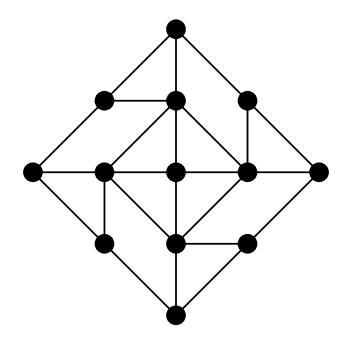
\includegraphics[scale=0.3]{02_crossover_gadget}
      \caption{Crossover gadget.}
      \label{img:crossover_gadget}
    \end{wrapfigure}

  \strut{}

  Построим гаджет, исправляющий пересечения рёбер (рис \ref{img:crossover_gadget}), при раскраске в 3 цвета цвета противоположных внешних вершин совпадают (и все пары раскрасок существуют). Воткнём такой гаджет на место каждого пересечения рёбер. Так как рёбер линейно от числа вершин.

\end{adjustbox} 

\end{reduction}

\begin{problem}(\s{$H$-coloring})\\
    Даны два графа $G$ и $H$, проверить, существует ли гомоморфизм из $G$ в $H$. 
    (гомоморфизм~--- отображение $g\colon G \to H$, т.ч. $\forall (u, v) \in E(G), (g(u), g(v)) \in E(H)$)\\

\end{problem}

\begin{remark}
\s{Coloring}~--- потому что если взять в качестве $H$ $k$-клику, получится просто \s{$k$-Coloring}. То есть мы красим вершины $G$ в цвета~--- вершины $H$~--- но не все пары цветов запрещены.
\end{remark}

\begin{remark}
Есть похожая задача~--- про миноры: проверить, что один граф является минором другого. И вот оказывается, что самым сложным минором является $k$-клика, её можно искать только за $k^{\Omega(k)}$.
\end{remark}

\begin{problem}(\s{$(2, k)$-CSP}) (Constraint satisfaction problem) \\
    Даны $n$ переменных, принимающих значения из алфавита размера $k$ и множество условий (предикатов) на двух переменных (любые условия, не только ДНФ).
\end{problem}

\begin{reduction}(\s{3-Coloring} $\xto{2^{\Omega(n)}, 2^{\Omega(n \log k)}}$ \s{$(2, k)$-CSP})\\
    По графу на $n$ вершинах построим $(2, k)$-CSP формулу на $\frac{n}{\log_3 k}$ переменных.\\
    Каждая переменная соответствует раскраске $\log_3 k$ вершин. А условия для каждой пары переменных запрещают противоречащие раскраски. Ну и понятно, нужно ещё запретить означивания переменных, в которых вершины из одного блока покрашены неправильно. 
\end{reduction}

\begin{statement}
\s{$H$-Coloring}~--- частный случай \s{$(2, k)$-CSP}.
\end{statement}

\begin{proof}
Означивание переменной соответствует ``цвету'' вершины. И единственные предикаты, которые можем использовать, задаются матрицей смежности $H$.\\
Заметим, что из этого факта вытекает, что \s{$3$-Coloring}~--- также частный случай \s{$(2, k)$-CSP}, в нём используется только предикат $\neq$.
\end{proof}

\begin{reduction}(\s{List $H$-Coloring} $\xto{2^{\Omega(n \log k)}, 2^{\Omega(n \log k)}}$ \s{$H$-Coloring}), где $k = |V(H)|$~\cite{Cygan2017} (скетч)\\
Пример: \s{List $3$-Coloring} $\to$ \s{$3$-Coloring}. Создадим треугольничек~--- ``палитру''~--- и соединим вершины, в которых запрещены какие-то цвета с соответствующими вершинами треугольничка.\\
Рассмотрим такой гаджет. Его понт в том, что при любом гомоморфизме центр переходит в центр. Чтобы работало и при большом $H$ (и не коллизилось с другими вершинами, засунем в центр клику $K_{k + 3}$).

\begin{figure}[H]
  \centering
  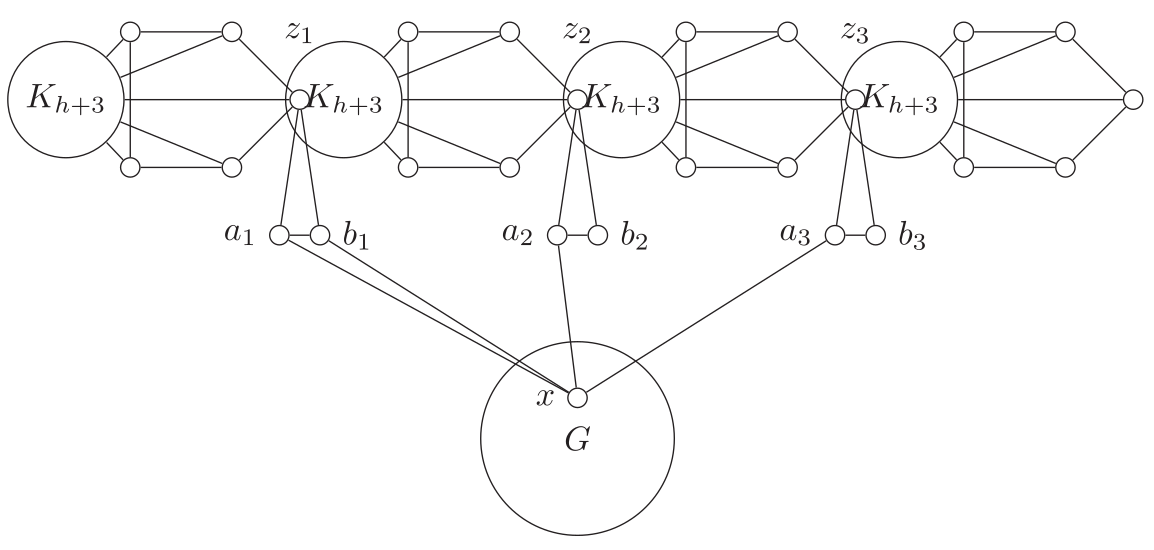
\includegraphics[scale=0.3]{02_list_h_coloring_gadget_worm}
  \caption{Пример гаджета для $k=3$, и вершины $x$, т.ч. $L(x) = \{1 \}$}
  \label{img:list_h_coloring_gadget_worm}
\end{figure}


Теперь сцепим $k$ таких гаджетов в цепочку. К каждому гаджету подвесим по две вершинки $a_i$ и $b_i$, это наша ``палитра''. Теперь вершинку графа $G$ соединим с $a_i$, и если её нельзя красить в $i$-ый цвет ещё и с $b_i$ (рис.~\ref{img:list_h_coloring_gadget_worm}). Аналогично соединяем с ``палитрой'' граф $H$. Примерно понятно, почему это работает (но тут скетч, так что строго не будет).


\end{reduction}


\begin{statement}\label{lm:lemma_3_2}~\cite{Cygan2017} 

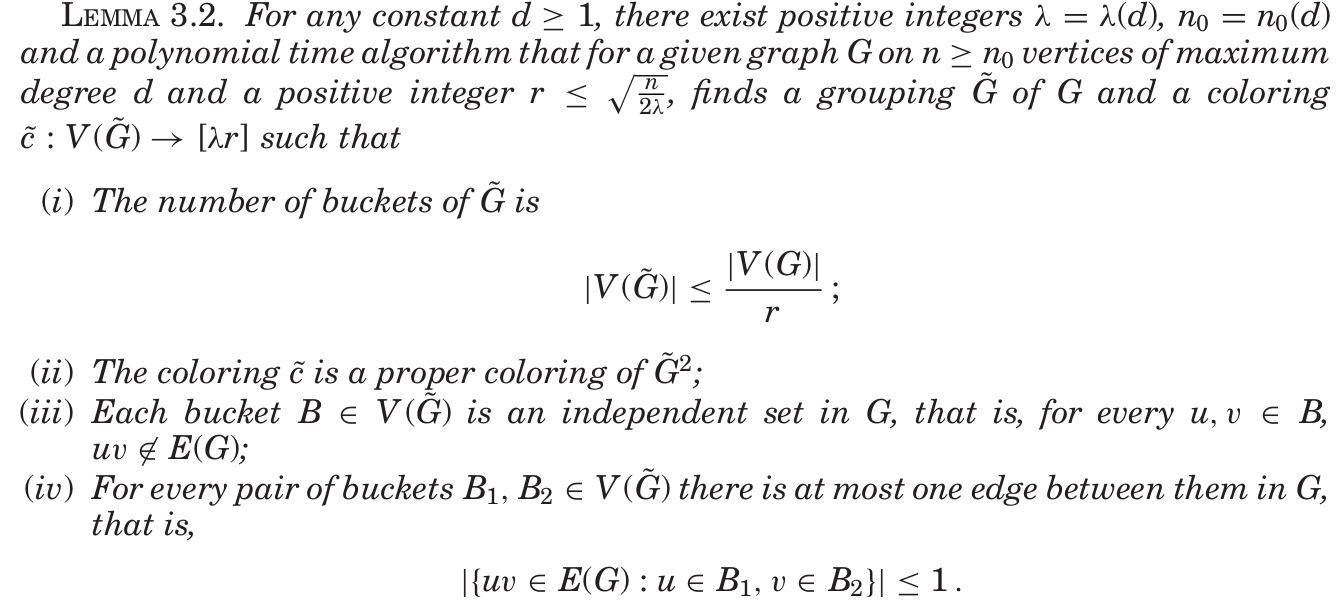
\includegraphics[scale=0.3]{02_lemma_3_2}
    
\end{statement}


\begin{reduction}(\s{Bounded Degree 3-Coloring} $\xto{2^{\Omega(n)}, 2^{\Omega(n \log k)}}$ \s{List $H$-Coloring}), где $k = |V(H)|$.\\

Хотим построить сведение примерно как для \s{$(2, k)$-CSP}~--- разбить вершинки на блоки, сжать блоки и решить \s{$H$-Coloring} для сжатого графа. Проблема в том, что мы не можем прослеживать связи между вершинами из разных блоков. Поэтому сведение будет более хитрым и потребует ``фактов из теории графов''.

Возьмём разбиение из утв.~\ref{lm:lemma_3_2} и его раскраску (будет говорить, что она задаёт не цвета, а лейблы, цвета~--- в исходном \s{3-Coloring}'е). Блоки образуют независимые множества и между двумя блоками не более одного ребра. Более того, так как раскраска переносится на $\widetilde{G}^2$, то для каждого блока все его соседи разных лейблов.

Для блока зададим 4-ичный вектор длины $\chi(\widetilde{G})$. На $t$-ой позиции этого вектора запишем цвет (в \s{3-Coloring}'е) соседа этого блока с лейблом $t$ (или 0, если такого нет). Тогда вершина в $H$ задаёт лейбл блока и кодировку. \s{List $H$-Coloring}'ом (частью про \s{List}) добиваемся того, что блок отображается только в свой лейбл. Соединяем в $H$ вершины, раскраски которых согласованы ($\phi_a (b) \neq \phi_b (a) \vee \phi_a (b) \phi_b (a) = 0$).

Теперь оценим время. Выберем размер блока равным $r$, тогда $|V(\widetilde{G})| \le \frac{n}{r}$, $|V(H)| \le \chi(\widetilde{G}) 4^{\widetilde{G}} = \O(r 4^{\O(r)})$. Выбрав $r = \O(\log n)$ получаем $|V(G)| = \O(\frac{n}{\log n})$, $|V(H)| = n^{\O(1)}$.

\end{reduction}

\begin{problem}(\s{Subgraph Isomorphism})
Даны графы $G$ и $H$, проверить, является ли $H$ подграфом $G$.
\end{problem}

\begin{reduction}(\s{$H$-Coloring} $\xto{2^{\Omega(n \log n)}, 2^{\Omega(n \log n)}}$ \s{Subgraph Isomorphism})\\
Переберём $a_i, \sum\limits_{i=1}^{|V(H)|} a_i = |V(G)|$~--- сколько вершин $G$ отобразится в $i$-ую вершину $H$. Продублируем $i$-ую вершину $H$ $i$ раз, поищем изоморфизм из $H$ в $G$. Так как неупорядоченных разбиений на слагаемые будет не более $2^{|V(G)|} = 2^{n}$ получили нужную оценку.

\end{reduction}

\subsection{Семинар}

\begin{exerc}
    $\forall \alpha > 0$ построить $(2^n, n^{1 + \alpha})$ fg-сведение \s{Ham Cycle} $\to$ \s{3-Sum}
\end{exerc}

\begin{problem}(\s{Max Inner Product})\\
    Даны $2$ набора $A$ и $B$ из $n$ векторов из $\{0, 1\}^d$, где $d = o(n)$. Найти $\max \{ \langle a, b \rangle | a \in A, b \in B \}$.
\end{problem}
    
\begin{exerc}
    Покажите, что \s{Max Inner Product} не решается за время $\O(n^{2 - \eps})$ под \s{SETH}.
\end{exerc}

\begin{exerc}
    Покажите оценку в $2^{\Omega(n)}$ на \s{Bounded Degree 3-Coloring} ($\frac{|E(G)|}{|V(G)|} = n^{o(1)}$) под \s{ETH}.
\end{exerc}
% просто есть сведение с degree <= 4

\begin{problem}(\s{Cross Matching})
    Дан граф $G$ с разбиением вершин на две доли по $n$ вершин. Проверить, существует ли такое совершенное паросочетание $M$ в $G$, что концы каждого ребра паросочетания находятся в разных долях и $G/M$ (стянутые рёбра) образует клику.
\end{problem}

\begin{exerc}\cite{Fomin2021}
    Покажите оценку в $n^{\Omega(n)}$ на задачу \s{Cross Matching} под \s{ETH}.
\end{exerc}





\pagebreak

\bibliographystyle{apalike}
\bibliography{bib.bib}

\end{document}
